% This is samplepaper.tex, a sample chapter demonstrating the
% LLNCS macro package for Springer Computer Science proceedings;
% Version 2.20 of 2017/10/04
%
\documentclass[runningheads]{llncs}
%
\usepackage{float}
\floatstyle{ruled}
\newfloat{algorithm}{htbp}{loa}
\floatname{algorithm}{Algorithm}
\usepackage{natbib}
\usepackage{graphicx}
\usepackage{xcolor}
\usepackage{amsmath}
\usepackage{amssymb}
\usepackage{algorithm}
\usepackage{algpseudocode}
\usepackage{subcaption}
\usepackage{multirow}
\usepackage{booktabs}
\usepackage{longtable}
\usepackage{hyperref}
\usepackage{textcomp}
\usepackage{enumerate}

\usepackage{array}
\newcolumntype{x}[1]{>{\centering\arraybackslash\hspace{0pt}}p{#1}}

\newcolumntype{C}[1]{>{\centering\arraybackslash}m{#1}}

\newcommand{\RNum}[1]{\uppercase\expandafter{\romannumeral #1\relax}}

% For japanese character for drawing kaomoji
\usepackage{tikz}
\newcommand{\shrug}[1][]{%
	\begin{tikzpicture}[baseline,x=0.8\ht\strutbox,y=0.8\ht\strutbox,line width=0.125ex,#1]
	\def\arm{(-2.5,0.95) to (-2,0.95) (-1.9,1) to (-1.5,0) (-1.35,0) to (-0.8,0)};
	\draw \arm;
	\draw[xscale=-1] \arm;
	\def\headpart{(0.6,0) arc[start angle=-40, end angle=40,x radius=0.6,y radius=0.8]};
	\draw \headpart;
	\draw[xscale=-1] \headpart;
	\def\eye{(-0.075,0.15) .. controls (0.02,0) .. (0.075,-0.15)};
	\draw[shift={(-0.3,0.8)}] \eye;
	\draw[shift={(0,0.85)}] \eye;
	% draw mouth
	\draw (-0.1,0.2) to [out=15,in=-100] (0.4,0.95); 
	\end{tikzpicture}}

\setcitestyle{square}

\begin{document}
%
\title{An Evolutionary Approach to Automatic Keyword Selection for Twitter Data Analysis\thanks{Supported by Public Health England.}}
%
\titlerunning{Automatic Keyword Selection for Twitter Data Analysis}
% If the paper title is too long for the running head, you can set
% an abbreviated paper title here
%
\author{Oduwa Edo-Osagie\inst{1} \and Beatriz De La Iglesia\inst{1} \and Iain Lake \inst{1}\and Obaghe Edeghere \inst{2}}
%
\authorrunning{O. Edo-Osagie et al.}

\institute{University of East Anglia, Norwich, United Kingdom\\ 
	\email{\{o.edo-osagie, i.lake, b.iglesia\}@uea.ac.uk}\\ \and
	Public Health England, Birmingham, United Kingdom\\
	\email{obaghe.edeghere@phe.gov.uk}
}

\maketitle              % typeset the header of the contribution
%
\begin{abstract}
In this paper, we propose an approach to intelligent and automatic keyword selection for the purpose of Twitter data collection and analysis. The proposed approach makes use of a combination of deep learning and evolutionary computing. As some context for application, we outline the proposed algorithm using the case study of public health surveillance over Twitter, which is a field with a lot of interest. In doing so, we also describe an optimization objective function particular to the keyword selection problem, as well as metrics for evaluating Twitter keywords, namely: \textit{reach} and \textit{tweet retreival power}, on top of traditional metrics such as \textit{precision}. In our experiments, our evolutionary computing approach achieved a tweet retreival power of \textbf{0.55}, compared to \textbf{0.35} achieved by the baseline human approach.

\keywords{Twitter \and Evolutionary Computing \and Syndromic Surveillance \and Social Media Sensing}
\end{abstract}
%
%
%
\section{Introduction}\label{Intro}
Syndromic surveillance can be described as the real-time (or near real-time) collection, analysis, interpretation, and dissemination of health-related data, to enable the early identification of the impact (or absence of impact) of potential human or veterinary public health threats that require effective public health action \cite{I_REF11}. As syndromic surveillance is concerned with the detection and understanding of public health threats, there is interest in rich, interesting and efficient data scources. De Quincey  and Kostkova \cite{I_REF15} introduced the potential of Twitter in detecting outbreaks. The amount of real-time information present on Twitter, either with regards to users reporting their own illness, the illness of others or reporting confirmed cases from the media, is both rich and highly accessible.

Twitter syndromic surveillance, like all other Twitter analysis applications, requires the collection of Tweets. This collection usually involves specifying some filtering criteria. The simplest and most commonly used criteria is filtering by keyword. In any Twitter analysis application, choosing the right set of keywords can have a big impact on the system as it controls which Tweets are collected and observed. Choosing keywords that are too precise and strict will result in our system collecting mostly relevant Tweets, but also simultaneously only observing few Tweets, which will most likely only be a small sample of the relevant Tweets available. Conversely, choosing keywords that are too broad will result in our system observing a great deal of Tweets, most of which will not be relevant. Therefore, selecting the right keywords is an important and difficult task. 

In this paper, we propose an intelligent and automatic approach to effective keyword selection. We leverage evolutionary algorithms and machine learning to quantify and distinguish semantic information in keywords, allowing us to select automatically select the best keywords to collect Tweets relevant to our application. For the sake of comparison, we also discuss a manual method of keyword selection, carried out by humans, and use this as a baseline in our experiments. We found that our automatic keyword selection algorithm was able to outperform the manual, human approach.


\section{Twitter Keyword Selection and Related Work}\label{keyword-selection}
Before we begin thinking about automatic keyword selection, we must first take a look at how keyword selection normally occurs. While this process might differ based on the purpose of the data collection, it will typically involve some domain knowledge relating to the purpose of the data collection. However, in addition to this, it is often useful to keep in mind that language on Twitter is usually very informal and colloquial. This must also be taken into account when selecting a set of keywords for any purpose. For syndromic surveillance, our goal when selecting keywords for collection was to choose keywords which may be relevant to our particular syndrome of interest. We worked in conjunction with experts from Public Health England (PHE), to create a set of formal terms that may be connected to the specific syndrome under scrutiny. This set of keywords was then further expanded using synonyms from thesauri and the urban dictionary\footnote{\url{https://www.urbandictionary.com}}. Urban dictionary is a web resource which serves as an encyclopedia of sorts for slangs, so it was used to account for informal language that may occur in Twitter.  

Much of the existing literature on keyword selection revolves around marketing and advertising efforts. Some researchers have looked at keyword selection as a feature selection problem \cite{HREF1}. Others have taking a classification point of view. For example, \cite{HREF2} applied a CNN to classify keywords as good or bad in order to maximaize advertising campaigns. More recently, with the influence of deep learning in natural language processing and the rise of deep word embeddings, such methods have seen a growing interest in keyword selection. \cite{HREF3} made use of Word2Vec embeddings to select keywords for websites using semantic similarity. In fact, similar to our work, \cite{HREF4} work towards the problem of social media analysis, making use of GloVe embeddings to infer keywords which can be used to find online trolls on social media. The problem with the solutions provided by a lot of the existing research, is that they assume that all similar keywords under a concept (such as asthma, for example), will collect relevant documents. They also assume that the addition of keywords will not dilute the quality of the collected data, just because they are all similar. However, this is not always the case. For this reason, we go further and attempt to optimize the set of keywords selected in such a way that confirms the above assumptions. 

\section{Evolutionary Automatic Keyword Selection for Twitter Data Analysis}
We propose a two-stage approach which makes use of deep learning and evolutionary optimization. The input to the system is a small initial set of reasonable keywords. Deep word embeddings are trained on a text corpus with a subject domain related to the task for which the keywords are intended. We make use of GloVe \cite{REF13} word embeddings which capture sematic meaning of words from observed context. Using these embeddings, we expand the initial input keyword set with words/phrases which are semantically similar or related to the input keywords. This expanded set of keywords then forms our candidate set which makes up our problem space from which we attempt to select the optimal subset to be used for Twitter data collection and analysis.

The task of keyword selection is modelled as an optimization problem. Each possible set of keywords is seen as a candidate solution and the goal is to find the optimal solution. In this approach, we make use of Particle Swarm Optimization (PSO) which is an evolutionary algorithm based on swarm intelligence put forward by J. Kennedy in 1995 \cite{K_REF7}. Loosely speaking, we model each potential set of keywords as a particle in the swarm. Each particle is moved around the search space with some velocity, which is influenced by its known best position, as well as the best positions found by other members of the swarm. 

\subsection{Stage \RNum{1}: Obtaining the Candidate Set of Keywords}
The first stage involves producing a larger set of candidate keywords, $C$, from which our optimal set will be selected. This is done by expanding the input query set, $I$, using deep word ebeddings as mentioned above. Word embeddings (sometimes referred to as word vectors) are a powerful distributed representation of text learned using neural networks that have been shown to perform well in similarity tasks \cite{REF19}. They encode semantic information of words in dense low-dimensional vectors. There are many different ways to learn word embeddings \cite{REF13,REF14,REF15}. After learning, an embedding matrix $X$ of size $|V| \times d$ is produced where $V$  is the set of all the words in our vocabulary and $d$ is the dimension of each word embedding. For this work, we built GloVe embeddings \cite{REF13} from a dataset of 5 million unlabelled Tweets collected without any keyword limitations. The trained GloVe embeddings allow our system to get an understanding of Twitter language and vernacular, as our application of choice is Twitter data analysis. For each word in our input, $I$, we obtain the $n$ most similar words/phrases. These are estimated as the $n$ closest vectors to the query word vector in the embedding space. We make use of cosine distance as our distance measure for estimating similarity. 

\subsection{Stage \RNum{2}: Applying Particle Swarm Optimization to Keywords}
We model the keyword selection task as an optimization problem. Here an individual or particle or solution is a set of keywords. In this problem, the goal is to find the set of keywords that provide the maximum (or minimum) of some objective function. While the obvious solution to such a problem would be simply to check each possible solution in the search space and select the best, this is not often feasible. This is die to the fact that as the problem space grows, the computational complexity increases exponsentially with it, making brute force search approaches a lot less feasible. PSO solves this problem by making use of a set population of particles, where each particle is a potential solution. Fig \ref{fig:particle-space} shows an illustration of the particles in a problem space. These particles are then set loose to explore the search space in order to find an optimal solution. They tend to swarm and form clusters in optimal regions of the problem space.
\begin{figure}[h!]
	\centering
	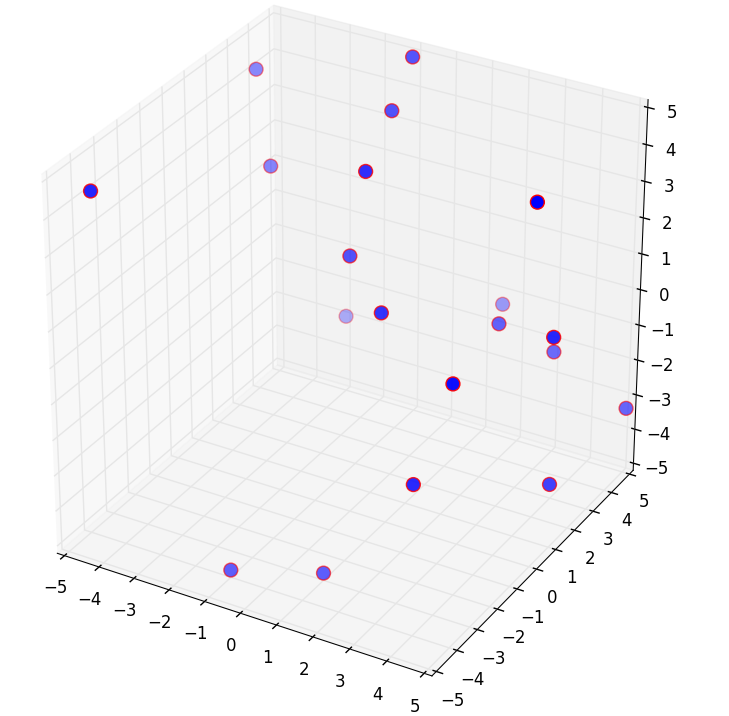
\includegraphics[scale=0.3]{Images/particle_space.png}
	\caption{Illustration of PSO particles in a search space}
	\label{fig:particle-space}
\end{figure}
We now look towards how we can model the keyword selection problem using PSO. Following the construction of the candidate keyword set $C$ as described above, we encode each keyword contained within it as a unique integer ranging from $1$ to $|C|$. With this, we can now represent a set of keywords as a vector of integers, $k$, where each integer in the vector maps to a keyword in $C$. The size of $k$, denoted as $D$, must be determined before-hand and equates to the maximum size of the desired final optimal keyword set. Additionally, while values of $1$ to $|C|$ represent keywords, a value of zero will be used to represent the absence of a keyword. With this, when keyword vectors are mapped back to keyword sets, it will be possible to have sets of varying sizes (of up to $|k|$). Having developed a way to represent a set of keywords as a vector, we can also represent a set of keywords as a particle, as a particle is represented by a vector. With this, we can apply PSO to our candidate set, $C$, to intelligently and automatically select a set of keywords.

We start by randomly initializing a population of particles (i.e. keyword sets) from $C$. In essence, we create a set number of random vectors of size $D$, with values ranging from $0$ to $|C|$. Each particle possesses a \textit{\textbf{position}}, $x$ and a \textit{\textbf{velocity}}, $v$, and keeps track of the best position it has found, that is, its ``personal best'' or \textit{\textbf{pbest}}. The system keeps track of the ``global best'' or \textit{\textbf{gbest}}, which is simply the best position that has ever been found by any particle. The position of the $i^{th}$ particle, $x_i = (x_i^1, x_i^2, x_i^3, ... x_i^D)$. The particles are all moved around the search space, with their positions updated based on their velocities, $pbest$ values and $gbest$. More formally, after each iteration at time $t$, the position of the $i^{th}$ particle is updated according to equation \ref{eqn:position} 
\begin{equation}
	x_i^{t+1} = x_i^t + v_i^{t+1}
	\label{eqn:position}
\end{equation}
The velocity of the particle, $v_i^{t+1}$, (at time $t+1$) used to update its position can be computed as shown in equation \ref{eqn:velocity} where $\omega$ is the inertia coefficient, $c_1$ and $c_2$ are acceleration coefficients and $r_1$ and $r_2$ are random floating point values between 0 and 1.
\begin{equation}
	v_i^{t+1} = \omega v_i^t + c_1r_1(pbest - x_i^t) + c_2r_2(gbest - x_i^t) 
	\label{eqn:velocity}
\end{equation}
There are three main components to the way the velocity of a particle is updated:
\begin{itemize}
	\item \textit{\textbf{Inertia Component:}} This component is intended to keep the particle moving (or not moving) in the direction it is headed, and is controlled by $\omega$. Lower values of $\omega$ will speed up convergence while higher values encourage particle exploration of the search space \cite{K_REF3}.
	
	\item \textit{\textbf{Learning Component:}} This component controls the size of the step a particle takes towards its next position in exploring the search space. It is controlled by the coefficient, $c_1$ \cite{K_REF4}. 
	
	\item \textit{\textbf{Social Component:}} This component implements swarm mentality, and causes a particle to move towards the best regions the swarm has discovered so far. It is controlled by $c_2$  \cite{K_REF4}.
\end{itemize}

Largely speaking, the particles in the swarm explore the search space based on the $pbests$ and $gbest$ within the swarm. These values are computed for a particle's position using the objective function, $Z$. Our goal is to minimize the value of the $Z$, which represents the underlying desire of the swarm system. It is the function to be optimized. We make use of an objective function that is particular to the task of selecting a keyword set. We wish to maximize the number of relevant documents (or Tweets in our application scenario) and minimize the number of irrelevant documents collected by a set of keywords. However, we don't wish to achieve this by being too selective and only collecting very few documents. Our goal is a combination of the relevancy of the Tweets we collect and the volume of Tweets we collect. Both of these figures are important to us. As such, we developed an objective function that belies this. The objective function, $Z$, is computed as the mean of two terms, $\alpha$ and $\beta$. $\alpha$ is the \textit{\textbf{irrelevance factor}} shown in equation \ref{eqn:alpha}, while $\beta$ is the \textit{\textbf{retrieval factor}} shown in equation \ref{eqn:beta}.
\begin{equation}
	\alpha = \sum_{i=1}^D (\frac{\sum_{j=1}^{|T|}k[i] \in T[j]}{\sum_{j=1}^{|T|}T[j] == irrelevant})
	\label{eqn:alpha}
\end{equation}
\begin{equation}
	\beta = \sum_{i=1}^D (1 - (\frac{\sum_{j=1}^{|T|}k[i] \in T[j]}{|T|}))
	\label{eqn:beta}
\end{equation}{}
$Z$ is computed as:
\begin{equation}
	Z = \frac{\alpha + \beta}{2}
	\label{eqn:objective}
\end{equation}{}

Finally, putting this all together, PSO keyword selection can be carried out by iterating over the following steps:
\begin{enumerate}
	\item The objective function is computed by each particle for their current position.
	\item Each particle updates their $pbest$ and the $gbest$.
	\item Each particle is moved once their velocity and position are updated, using the $pbest$ and $gbest$ values computed from the objective function.
\end{enumerate}
The steps are repeated either until the values converge, or a predetermined maximum number of iterations is reached.


\section{Experiments and Results}
% broad comparison like computational costs, generalizative potential etc.
% which is better
We were interested in understanding if our proposed approach solved the task of intelligent and automatic keyword selection at all, and if so, also understanding how well it did so. We implemented and ran Tweet collections for the asthma/difficulty breathing for syndromic surveillance using our keyword selection approach and the typical manual approach, for a baseline. We undertook two sets of collection periods. The first collection period was a sort of ``validation'' collection period, inspired by the training/validation/test splits adopted when building machine learning models. This validation collection period was used by our proposed approaches to automatically generate keywords. These generated keywords were subsequently utilized in a second collection period, intended to allow us to measure how well the generated keywords perform. This can be seen as our ``test'' collection period. Our validation collection period ran for a seven day period from the  24\textsuperscript{th} of May, 2019 till the 1\textsuperscript{st} of July, 2019. Our test collection period ran for a further seven day period from the 1\textsuperscript{st} of July, 2019 till the 8\textsuperscript{th} of July, 2019. Only the PSO-based approach was involved in the validation collection period, as the baseline approach does not need any data for setting it up. During the test collection period however, both approaches are involved.

One caveat to consider is that even though the evaluatory Tweet collections were performed simultaneously in parallel, due to the workings of the Twitter API, there is no guarantee that both systems will be exposed to the exact same Tweets at the exact same time. This is because of the fact that the Twitter streaming API only offers a sample of the entire real-time stream, the percentage of which will vary depending on the activity loads at the time. Despite this limitation of the free Twitter API, we should still be able to get some picture of how well our approaches perform. In this section, we describe the experimental setup for each approach, including the baseline standard keyword selection approach. After that, we present and discuss the results we obtained.

\subsection{Experimental Setup: Baseline Approach}
The baseline approach involved working with a group of domain experts to come up with useful keywords and augmenting these keywords with some terms from the Urban Dictionary. We came up with a list of keywords which are included in the appendices. Using these keywords, we ran a Tweet collection during the test collection period, from the 1\textsuperscript{st} of July, 2019, till the 8\textsuperscript{th} of July, 2019. The validation collection period was not used for this part of the experiments as there was no automatic keyword generation, rendering such a period unnecessary.

\subsection{Experimental Setup: Particle Swarm Optimization-Based Keyword Selection Approach}
The standard keyword set used in the baseline approach was used as the seed input $I$ for creating the candidate set $C$. For each word in $I$, their five most similar words as inferred from our GloVe embeddings were added to the set. Using the candidate set of keywords, Tweets were collected during the validation collection period. At the end of this period, the PSO-based keyword generation algorithm was applied using the collected Tweets. We set our $D$, representing the maximum size of a keyword set to be 10. We made use of the PySwarm library of evolutionary algorithms to implement our PSO algorithm. Our setup had a swarm size of 100. After some experimentation, we set our $\omega$ to 0.8., and $c_1$ and $c_2$ to 1. This resulted in the following set of keywords being selected as the optimal arrangement: \textit{wheezing}, \textit{panting}, \textit{gasping}, \textit{puffing}, \textit{coudn't breathe}, \textit{wheeze}, \textit{asthma}, \textit{inhaler}, \textit{sore eyes}.
After obtaining the automatically selected keywords, we applied them during the test collection period, using them as query inputs.

\section{Results}
We utilized the set of keywords we obtained from our keyword selection algorithm as query inputs for Tweet collection. We also utilized the keywords obtained using the standard baseline approach. We applied the two distinct sets of keywords in parallel during our test collection period -  1\textsuperscript{st} of July, 2019, till the 8\textsuperscript{th} of July, 2019. We then analyzed the Tweets collected by each set of keywords in order to understand how useful each keyword set was. We assessed the keyword sets based on their information retrieval ability. A lot of the traditional information retrieval metrics do not translate well, or cannot be calculated for our problem. For example, recall, which measures the fraction of relevant documents retrieved cannot be calculated because we have no way of knowing the total amount of relevant Tweets out there. Because of this, we made use of a combination of traditional metrics and developed problem-specific metrics. These metrics are \textit{\textbf{precision}} and \textit{\textbf{reach}}.  

Precision is a popular information retrieval metric which represents the proportion of retrieved documents which are relevant. In such an information retrieval context, precision is calculated as:
\begin{equation}
	precision = \frac{|Relevant Tweets| \cap |Collected Tweets|}{|Collected Tweets|}
\end{equation}
In our scenario, precision measures the proportion of the collected Tweets which are relevant. When calculating the precision values for each keyword appraoch, we computed the precision over a random sample of the retrieved Tweets. We took random 2000-large samples of the Tweets colletected using each keyword selection approach and computed the precision from this sample. We did this because we wanted to manually label and count the number of relevant Tweets, instead of relying on one of our trained classifiers which are not perfect. Doing so allowed us to get an accurate and exact value for the number of relevant Tweets, and would not be feasible with the complete set of collected Tweets which are very large and would be incredibly time-consuming to manually label.

\textit{Reach} is a metric we developed to help us capture the ability of a set of keywords to retrieve as many Tweets as possible, relevant or not. This is important because while it is useful to collect relevant Tweets, if we only observe a small amount of Tweets, we cannot create a useful signal which is appropriately representative of the activity related to the syndrome of interest. As such, reach measures the quantity of Tweets a set of keywords is able to collect. This could be computed simply as the proportion of the general Tweet stream that is collected using a set of keywords. However, the inner workings of the Twitter API is unknown to us. To overcome any bias introduced by the API and any rate limits it may impose, we calculate the \textit{reach} of a set of keywords in relation to the simplest singular keyword possible. This can be formally represented as shown below:
\begin{equation}
	reach = \frac{|Collected Tweets|_{\hat{k}} - |Collected Tweets|_{K}}{|Collected Tweets|_{K}}
\end{equation}
$\hat{k}$ represents some arbitrary single unit keyword which is a simple and straightforward keyword. For example, in our scenario of \textit{asthma/difficulty breathing} surveillance, we make use of the keyword ``asthma'' as $\hat{k}$.

Finally, we combined the precision and reach metrics into one metric by taking their harmonic mean, similar to the $F$-measure. We term this combined metric, the \textit{\textbf{Tweet Retrieval Power (TRP)}}.
\begin{equation}
	TRP = 2 \frac{precision \times reach}{precision + reach}
\end{equation}
The TRP weights precision and reach evenly but similarly to the $F$-measure, it is possible to calculate variations of the TRP score which place different weights on precision and reach as below:
\begin{equation}
	TRP_\beta = (1 + \beta^2) \frac{precision \times reach}{\beta^2(precision + reach)}
\end{equation}
where $TRP_\beta$ measures the Tweet retrieval ability when $\beta$ times as much importance is placed on reach than precision.


\begin{table}
	\centering
	\begin{tabular}{ |c|c|c|c| } 
		\hline
		\textbf{Keyword Selection Approach} & \textbf{Precision} & \textbf{Reach} & \textbf{TRP} \\
		\hline
		Baseline Human Approach  & 0.23 & 0.75 & 0.35\\
		\hline
		PSO Approach  & 0.48 & 0.65 & 0.55 \\
		\hline
	\end{tabular}
	\caption{Performances of different approaches to keyword selection}
	\label{table:kw-analysis}
\end{table}

Table \ref{table:kw-analysis} shows the results observed at the end of our analysis. We found the PSO approach to have the best Tweet Retrieval Power. The PSO approach produced a fair improvements in precision over the baseline human approach. It also resulted in a decrease in reach however. The precision achieved by the PSO keyword selection approach is more than double that seen by the baseline. In addition, while the reach of the baseline approach is better than that of the PSO approach, the margin between them is not very large. Finally, all things considered, the total Tweet Retreival Power of the PSO approach is greater than that of the manual baseline approach, and appears to possess a reasonable balance of precision and reach.

\section{Discussion}
In this paper, we investigated hybrid approaches to intelligently and automatically selecting keywords for use in collecting data, using Tweets for syndromic surveillance as a case study. We proposed an evolutionary algorithm inspired method which modelled the keyword selection task as an optimization problem. It made use of Particle Swarm Optimization (PSO) to determine the optimal set of keywords. The proposed algorithm was implemented and applied to the task of collecting Tweets for the surveillane of the \textit{asthma/difficulty breathing} syndrome. For the sake of comparison, we also carried out a Tweet collection with keywords selected using a manual, human approach. We then evaluated the results of both approaches, making comparisons between them.

We found that the PSO-based method performed better, outperforming the manual, human approach by a fair margin. While we observed a fair increase in relevance (precision) using our automatic keyword selection algorithms, we saw the opposite when looking at the reach metric. The baseline human approach to curating keywords seemed to have the most reach. Despite this, the boost in precision offered by the automatic keyword selection algorithm meant that it outperformed the baseline approach, yielding a higher TRP value. However, it is also important to remember that while we tried to keep things constant in our experiments, applying each keyword selection approach in parallel during the same periods, we cannot guarantee that they were exposed to the same environments and Tweets as that is an issue dependent on the Twitter API. Studies have estimated that using the Twitter streaming API, users can expect to receive anywhere  from 1\% of the tweets to 40\% of tweets available in real-time, depending on the amount of activity at the time \cite{K_REF8}. 

While we have introduced this technique for the intelligent and automatic selection of keywords and used them for surveilling the syndrome of \textit{asthma/difficulty breathing}, this does not mean it does not generalize to other tasks. These techniques cannot only be applied for the purposes of surveilling other syndromes on Twitter, but also for any Tweet collection exercise, regardless of the purpose of said exercise. This is due to the fact that these techniques aim to maximize the relevance of collected Tweets to some query, together with the volume of Tweets collected. As long as there exists some defined query, the notion of ``relevance'' for its results must also exist. Because these are the main ideas behind our proposed approaches, they can be very easily adapted to any other problem and generalize very well.

While we have established that the PSO method collects better Tweets, it also runs in a very reasonable amount of time. This is because the time taken for each iteration is determined by how many particles the swarm contains and the dimension of each particle, as well as the computational resources available. Even with a mid-tier computer, a single iteration could never take longer than an hour in the absolute worst case. As such the PSO method is not only superior in terms of the quality of the keywords produced, but also in terms of the amount of time taken to produce said keywords.
%
% ---- Bibliography ----
%
% BibTeX users should specify bibliography style 'splncs04'.
% References will then be sorted and formatted in the correct style.
%
\bibliographystyle{splncs04}
\bibliography{ref}


\end{document}
